\section{Components}

\todo{Logical Architectural View}

For starters, we split the project into a number of smaller modular components, that, when put together, make up a product that solves the requirements. The purpose of this is to gain an overview of the pieces of functionality required for the product, and the dependencies between these. Each component will be regarded as a wholly modular piece of the product and will be tested separately from the rest. 

%Each component deals with only its own concerns

See figure \ref{fig:components} for the component diagram showing a separation of concerns into product components and their dependencies. On each component we've written the main functions that the component allows, abstracting away all low-level details. The arrows signify dependencies, e.g. that the manoeuvre-component requires the functions of the driving-component in order to work. 

\begin{figure}[ht]
    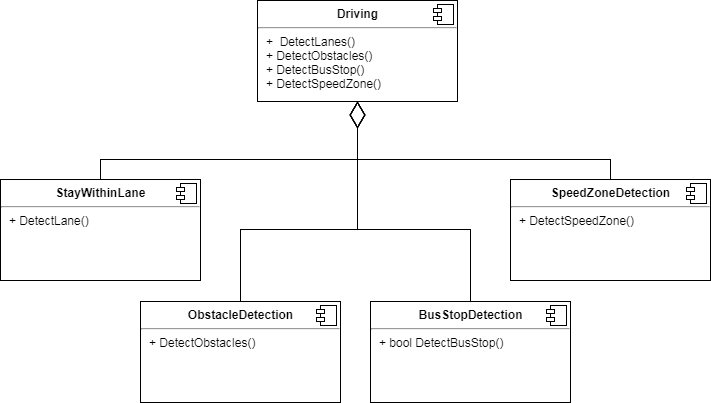
\includegraphics[width=\textwidth]{Images/Design/componentDiagram.png}
    \caption{Major components of functionality in the product; each component deals only with its own concerns}
    \label{fig:components}
\end{figure}
%Jeg er ikke overbevist om at ovenstående diagram er vildt vigtigt når vi nu alligevel har det nedenstående, dog giver det fint mening indtil videre

Note that the components refer not only to software, but also the physical design of the car. For instance, after we implement the driving component in software, we require a functioning LEGO-bus to test the software on. Only after this is done can we conclude whether the component works properly. Reason being that although the software logic might work as intended, incorrect sensor measurements, track/lane inconsistencies and similar need to be taken into account during programming, because otherwise, the product might not work as expected.

\subsection{Assumptions and Guarantees}
For now, we are imagining each component as a black box. What it contains is not of importance, only what it can do. Each component guarantees specific functionality as long as certain assumptions are met, see figure \ref{fig:assumptionGuarantee}. 

\begin{figure}[ht]
    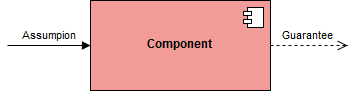
\includegraphics[width=\textwidth]{Images/assumptionGuarantee.png}
    \caption{The assumption-guarantee model}
    \label{fig:assumptionGuarantee}
\end{figure}

Most of the assumptions are made for the sake of simplicity in order to not delude the design with unnecessary detail. In this section, we will specify assumptions and guarantees that are not immediately obvious. Other, common assumptions, like the fact that the bus needs gravity to drive properly, will also still be left implicit. The specifications will later be used for informing the creation of interfaces for the classes of the program. 

We will now further describe the major components in text.
\begin{description}
    %\item[Driving]
    
    \item[Obstacle Avoidance]
    We assume the obstacle is large and made out of material that can be detected consistently by the ultrasonic sensor. 
    
    \item[Stay Within Lane]
    The component assumes perfectly consistent road markings with no imperfections and unintentional holes. 
    
    \item[Cruise Control]
    We assume that the vehicle to follow drives at a speed that makes sense, e.g. not too slow to detect and not too quick to follow. 
    
    \item[Speed Zone Control]
    We assume that each different speed limit is marked with a single sign to be recognized by the nxtCam sensor. 
    
    \item[Manoeuvre]
    We assume that at any point where lane switching is allowed, lines will be replaced with dotted lines. 
    
    The component guarantees that it can park parallel to a bus stop with a maximum distance of 1 cm to the edge at any point. 

    \item[Stop Button]
    Although this fits less well with the reality, we will not be using a physical stop button inside the bus, because this will be tough to click. For this reason, the component assumes that it receives a Bluetooth signal, and will then ensure that the bus halts at the next stop.  
    
    \item[Detect Bus Stop]
    While there are many different types of bus stops, in reality, we assume that there is only a single bus stop design that we need to recognise using the nxtCam sensor. This will be specified during the implementation.
    
    
\end{description}